\subsection{Introducción}

Se requería una página web que pudiera recibir y gestionar los datos de cada módulo Solar Link, como también mostrar esos datos a nombre de un usuario. \\

Luego de una investigación en la que se evaluaron opciones como node.js (un framework o marco de trabajo en javascript) y django (un framework basado en python), se decidió usar django para el backend del proyecto. Esto debido a su amplia variedad de herramientas ya preparadas; la posibilidad de manejar bases de datos sin lenguaje SQL (escribiendo código en python que luego el framework traducía a SQL); el amplio nivel de soporte en internet: secciones de código ya armadas de ejemplo y la posibilidad de usar cualquier librería o módulo de python de terceros sin tener que hacer ningún cambio extra; los conocimientos previos de python por parte de los integrantes; y la posibilidad de utilizar bloques lógicos de python en código HTML, permitiendo cambiar las vistas de la página web con condiciones y bucles.\\

Luego de definir eso, se creó el repositorio de GitHub para poder trabajar en equipo en la página web y tener un registro de los avances. También se hizo una investigación profunda de django para saber cómo encarar el desarrollo y una futura aplicación de Android.\\


\subsection{Django}
Django es un framework (marco de trabajo) basado en python. Está centrado en tener herramientas que faciliten programar y unifiquen todo en el mismo lenguaje de programación. Se basa en el concepto MVC, o vista-modelo-controlador.\\

\begin{figure}[H]
    \centering
    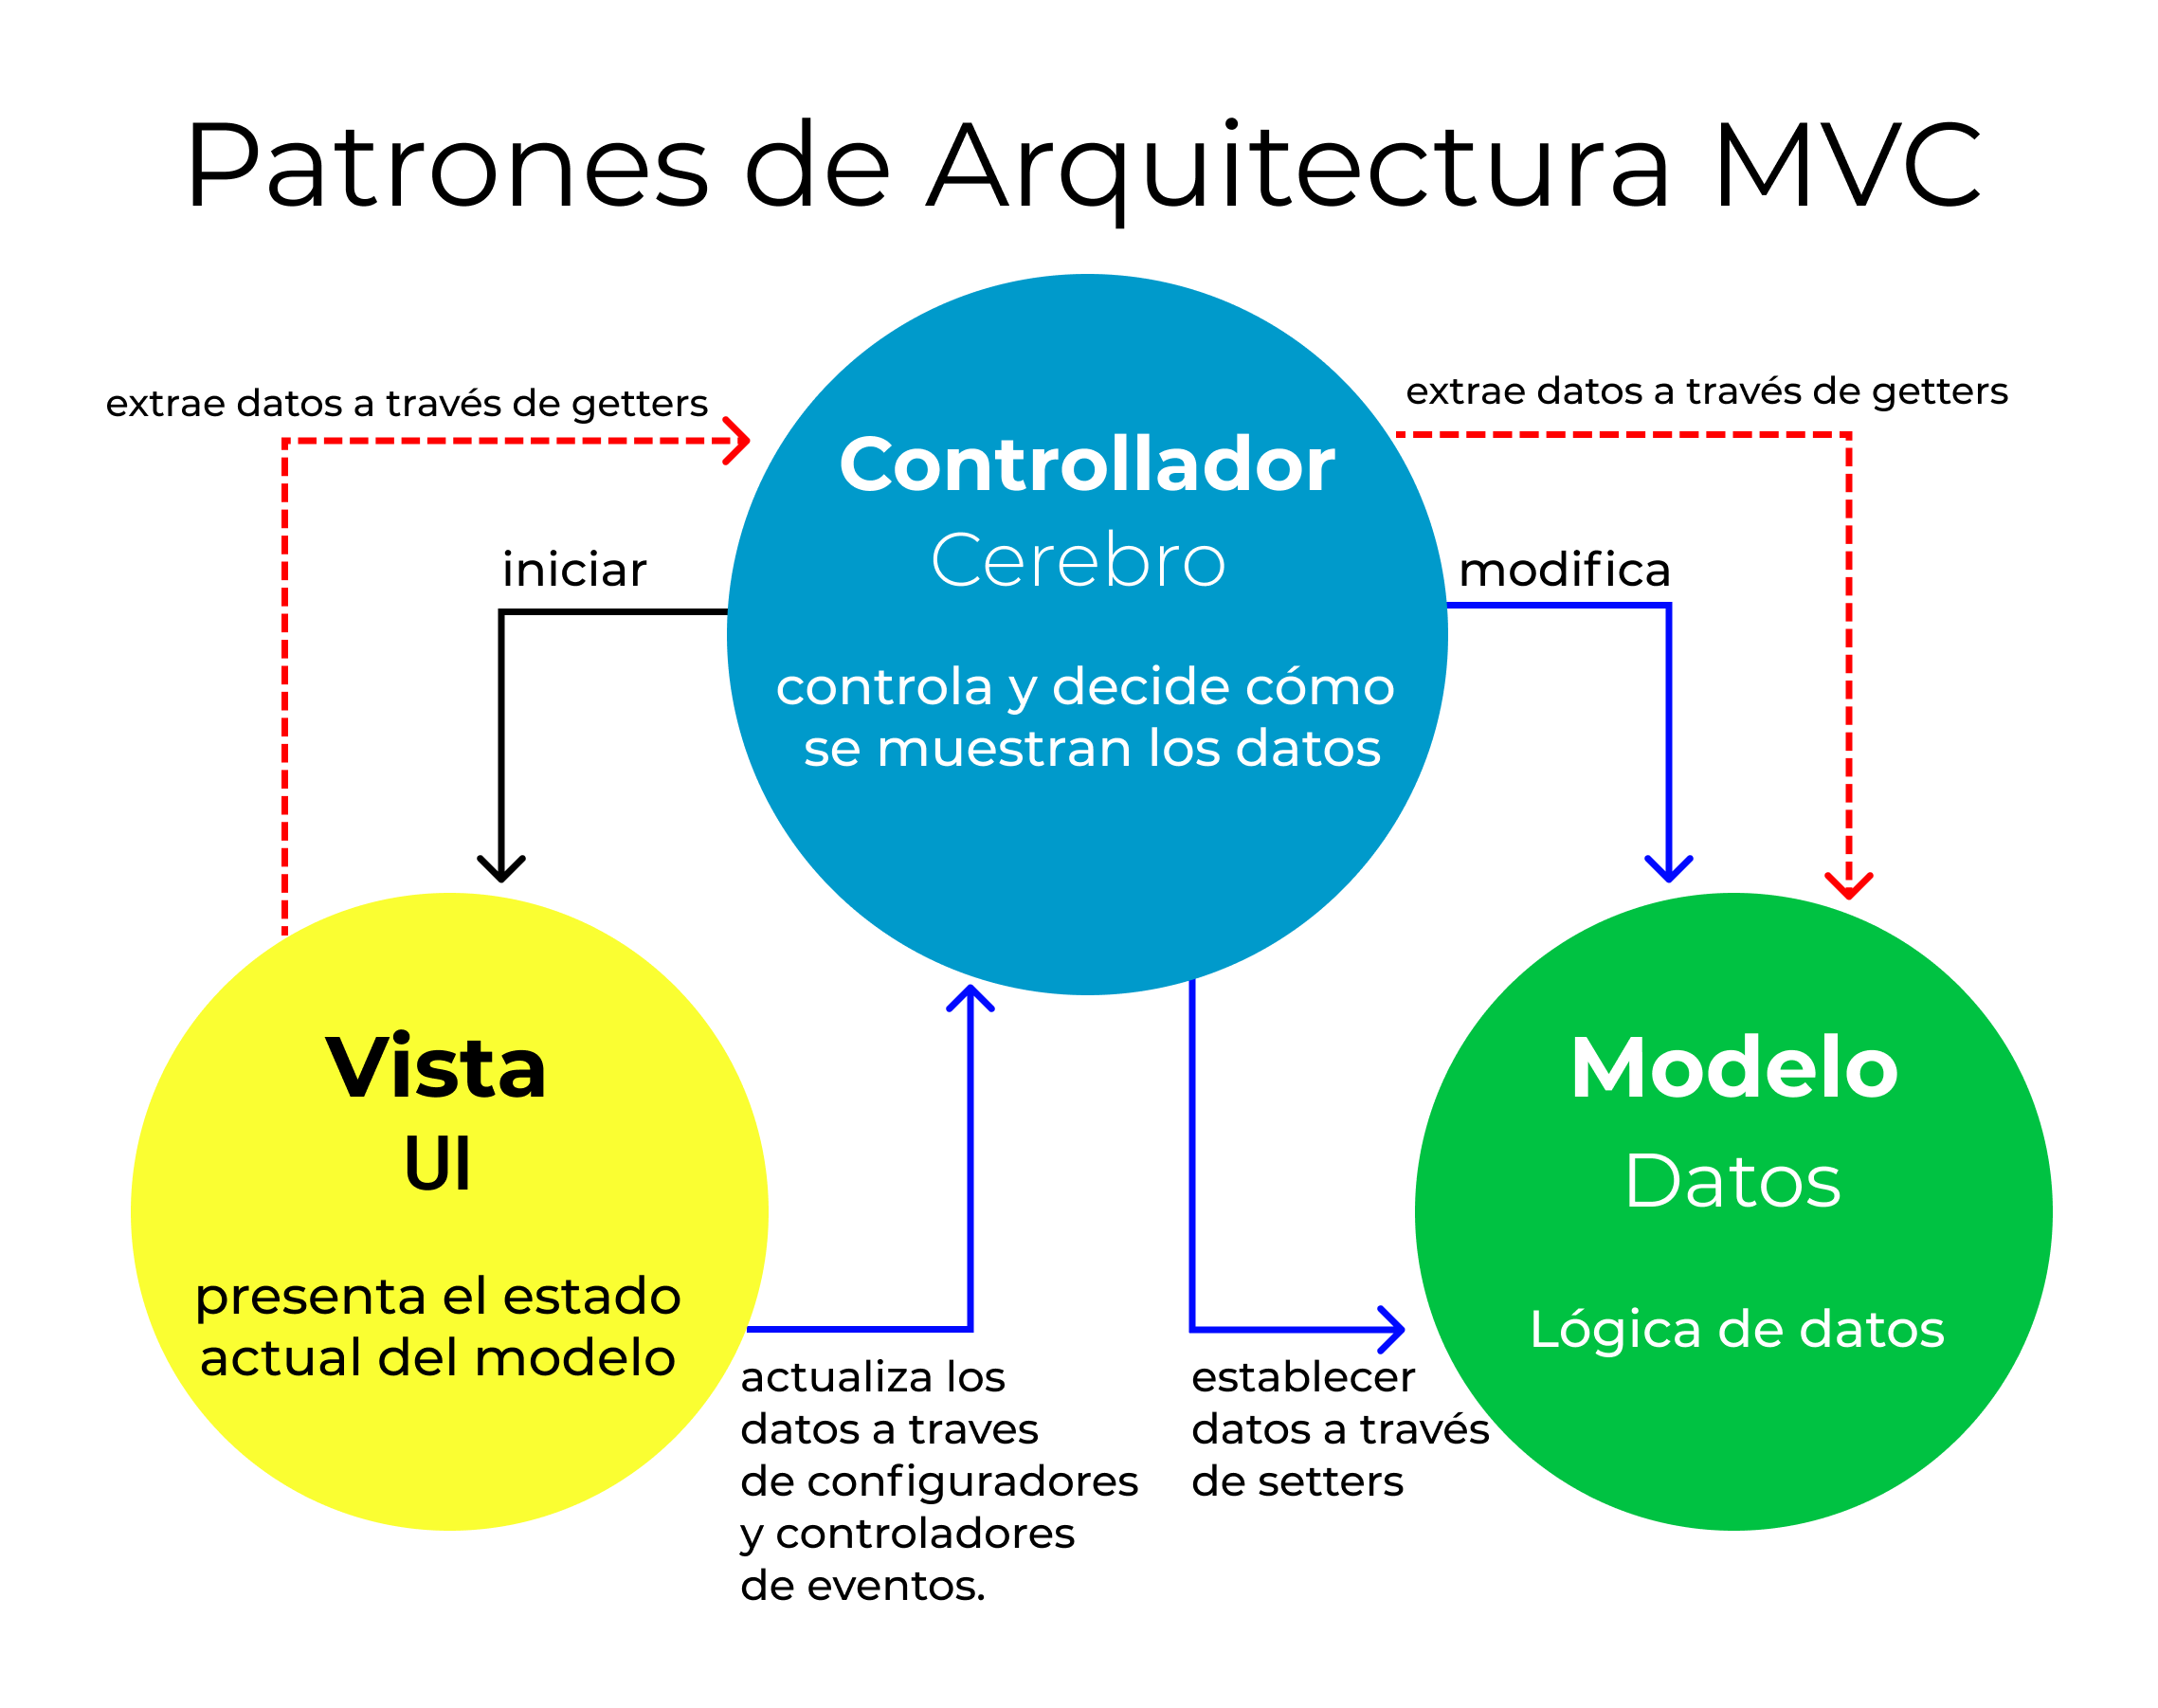
\includegraphics[width=1\linewidth]{web/MVC3.png}
    \caption{Lógica manejada en la página web.}
    \label{fig:arch-mvc}
\end{figure}

Aunque en Django a la vista se le llama template y al controlador se le llama vista.
Aquí, las vistas se ven representadas como funciones o clases que manejan lógica, reciben datos y retornan datos.\\

\begin{listing}[H]
\begin{minted}{python}
def geeks_view(request):
    # fetch date and time
    now = datetime.datetime.now()
    # convert to string
    html = "Time is {}".format(now)
    # return response
    return HttpResponse(html)
\end{minted}
\caption{Ejemplo de vista django}
\label{listing:vista-ejemplo}
\end{listing}

Los templates son HTML estándar, a los que se les puede combinar CSS y JavaScript. Lo novedoso aquí es el uso del django template language, donde se pueden integrar valores, funciones, condicionales y bucles que no son propios de HTML, permitiendo una mayor conexión entre la vista y el template.\\

\begin{listing}[H]
\begin{minted}{django}
Hello, {{ user.username }}.
\end{minted}
\caption{Ejemplo de un if en django template language en un HTML.}
\label{listing:django-template-ejemplo}
\end{listing}

Por último, los modelos son clases de python en la que se definen campos de SQL como si fueran atributos de la clase. Esto permite que Django procese y cree la base de datos automáticamente, sin que el usuario tenga que escribirle comandos en SQL. Luego, con ciertas funciones predefinidas del framework, se pueden añadir o borrar datos a la base.\\


\subsection{Módulos utilizados}

Una de las mayores ventajas de django es su amplia variedad de módulos hechos por terceros, prácticamente todo el material de python es compatible con este framework, y también existe una variedad de módulos que agregan funciones a django. Aquí se detallarán las que se utilizaron para el proyecto:\\

\subsubsection{BeautifulSoup}

Es un módulo de python que permite interactuar con HTML y tomar contenido de este. En el proyecto, se utilizará para tomar de las web nacionales los precios del KW/h de los cuadros tarifarios, y utilizarlos para estimar el costo de lo consumido por el hogar.\\

\subsubsection{Celery}

Es un módulo de python que permite correr funciones de python de forma paralela al código fuente; permitiendo así que las tareas pesadas, como la escritura en la base de datos, no retrasen la respuesta de la página web. \\

\subsubsection{django-compressor y django-libsass}

En django se trabaja con directorios fijos para el static (imágenes, CSS y JS), esto significa que cuando se llama a una imagen en el HTML, no se usan términos como “../static/img/imagen.png” sino que se usa el django template language para referirse a la carpeta static, que es única y se define en configuración. Un ejemplo es: {\% static “img/imagen.png” \%} (nótese cómo se omite la mención del directorio /static/, o el retorno hacia atrás, ya que django con el término static entre llaves, ubica automáticamente los archivos. Sin embargo, esto sólo aplica para HTML, si se requiere un llamado de static desde, por ejemplo, el CSS, de forma nativa no contamos con esta cualidad. Aquí entran los módulos django-compressor y django-libsass que, por medio de convertir los archivos CSS a SCSS, agregan funciones a este archivo como static() que funcionan como un equivalente a {\% static … \%}.

\subsubsection{Django-crontab}

Este módulo de django permite la ejecución de tareas paralelas cada determinado tiempo. Se utilizará para tareas como ordenar diariamente la base de datos y eliminar los tokens de cambio de contraseña y registro (se detallará más adelante).\\

\subsubsection{requests}

El módulo requests permite comunicarse por HTTP con, por ejemplo páginas web. Se utiliza para obtener el HTML de las páginas nacionales que luego se procesará con Beautiful Soup.\\

\subsubsection{secrets}

Este módulo de python permite generar bytes de dígitos aleatorios, tokens, etc. Se utilizará para crear los tokens (códigos de “x” dígitos que son necesarios para acceder a una pestaña, y se borran con el tiempo o tras su utilización) de cambio de contraseña y confirmación de registro.\\

\subsubsection{json}

Este módulo de python permite convertir JSONs a diccionarios y diccionarios a JSONs.

\subsection{Configuraciones del proyecto}

Existen muchos módulos y funciones propios de django que se utilizaron:
\begin{itemize}
    \item login\_required: permite hacer vistas solo accesibles por usuarios logueados en la plataforma.
    \item render\_to\_string: renderiza HTML a strings, útil cuando se quieren enviar mails desde el código.
    \item HttpResponse, JsonResponse: permiten que una vista responda con HTML o en formato JSON.
    \item render: Permite renderizar HTML que tiene django template language en él, y que las vistas devuelvan estos al ser llamadas.
    \item redirect: permite redireccionar desde una vista a otra.
    \item User: permite trabajar con la clase User, que es un sistema de usuarios preparado para django.
    \item auth: permite iniciar sesión a usuarios y validarlos.
\end{itemize}

\subsubsection{Directorio raiz}

El directorio raíz de la web se ve como en la figura \ref{fig:root-dir}. El proyecto completo puede encontrarse en \href{https://github.com/solarlink-ar/solarlink}{nuestro GitHub}.

\begin{figure}[H]
    \centering
    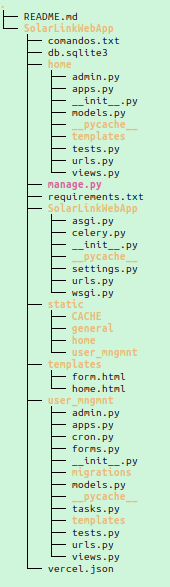
\includegraphics[width=0.18\linewidth]{web/imageedit_2_7842957095.png}
    \caption{Directorio raíz.}
    \label{fig:root-dir}
\end{figure}

Se puede notar que la carpeta raíz es SolarLinkWebApp, dentro de esta se encuentran: \\

\begin{itemize}
    \item El archivo manage.py (es el archivo base del proyecto, a partir de este se ejecutan todas las funciones y partes del código, y con este se inicia el servidor web, entre otros).
    \item db.sqlite3, es la base de datos, puede notarse que es en formato sqlite3.
    \item comandos.txt, es un archivo a modo de recordatorio de comandos de terminal necesarios para ejecutar el servidor y configurar el proyecto\\

\begin{listing}[H]
\begin{minted}{console}
            python3 manage.py runserver <IP:Puerto>
            celery -A SolarLinkWebApp worker -l INFO
            python3 manage.py crontab add 
            python3 manage.py crontab show
            python3 manage.py crontab remove
\end{minted}
\label{listing:comandos en terminal}
\end{listing}


    \item requirements.txt, contiene la lista de módulos usados en el proyecto. Este archivo sirve para instalar todos los módulos necesarios a la vez utilizando pip y apuntando hacia este archivo, y para que el servidor web sepa qué módulos son necesarios.

    \item vercel.json, es el archivo de configuración del servidor web que utilizamos.
    \item SolarLinkWebApp, aquí se encuentran los archivos generales de configuración del proyecto.
    \item home, aquí se encuentra el código fuente de la aplicación home, es decir, aquella que maneja las pestañas de inicio, explicación del proyecto y galería.
    \item user\_mngmnt, aquí se encuentra el código fuente de la aplicación user management, esta contiene el sistema de login, signup, posteo de datos desde la ESP32, página que muestra los datos, etc.
    \item static: Contiene todos los archivos de static (imágenes, CSS y JS).
    \item templates: contiene los templates generales que se pueden extender. En django se puede hacer un archivo HTML con “bloques a rellenar”, estos bloques después se rellenan en otro HTML que “extiende” al original. Esto permite hacer varias pestañas que son iguales, por ejemplo, en el pie de página y la barra superior; pero cambia el contenido del medio.

\end{itemize}

\subsubsection{Directorio SolarLinkWebApp/SolarLinkWebApp}

Aquí se encuentran los archivos principales de configuración, aquellos marcados con un “*” fueron editados y se les alteró el código, aquellos sin marcar no fueron alterados a partir de lo predefinido por django:\\

\begin{itemize}
    \item ASGI.py: se encarga de gestionar los procesos asíncronos del proyecto.
    \item WSGI.py: gestiona el servidor web.
    \item urls.py*: contiene los “path” (caminos, por ejemplo solarlink.ar\textbf{/galeria}, o solarlink.ar\textbf{/user/login}). En el listing \ref{urls.py_raiz} se detalla el código. Se definió que todos los path de la app home sean solarlink.ar/…, y todos los paths de user\_mngmnt sean solarlink.ar/user/… 
    \item celery.py*: el archivo de configuración de celery, aquí se define que los archivos que tienen las funciones que se ejecutarán en paralelo serán definidas en un archivo llamado tasks.py, y se le da permiso para buscar estos archivos adentro de las aplicaciones (home y user\_mngmnt).
    \item settings.py*: Contiene las configuraciones generales de django y los módulos. En el listing \ref{settings.py} se detallan las configuraciones editadas y añadidas al proyecto, que no vienen por defecto en el settings.py.
    \item \_\_init\_\_.py*: se definió la app de celery.
    
\end{itemize}

\subsubsection{Directorio templates}

Contiene el código de HTML de home y forms, útil como base para las pestañas de home y los formularios de login, signup, etc, de user\_mngmnt. En el listing \ref{home.html} se muestran ejemplos del head y la barra superior de home.html, a modo de ejemplo de cómo se puede aplicar el django template language.

\subsection{App home}

\subsubsection{Directorio home}
\begin{figure}[H]
    \centering
    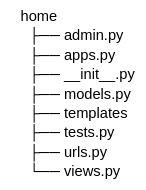
\includegraphics[width=0.25\linewidth]{web/Captura desde 2023-10-16 23-06-46.png}
    \caption{Directorio app home.}
    \label{fig:home-dir}
\end{figure}
\begin{itemize}
    \item urls.py: aquí se definieron los paths de esta app y se direccionaron a una vista determinada. En el listing \ref{urls.py_home} se encuentra el código.
    \item views.py: aquí se definieron las vistas, que en este caso solo renderizan el HTML con django template language. Estos HTMLs al igual que los del resto del proyecto se detallarán en la sección de frontend. En el listing \ref{views.py_home} se encuentra el código del views.py.
    \item Carpeta templates: contiene los HTMLs que se insertan en el template general home.html, y el HTML de galería.
\end{itemize}

\subsubsection{Views y frontend}

Las vistas que se renderizan en esta app son la de home y la de galería. Funcionan en relación a si el usuario está o no logueado, mostrando una pestaña distinta para cada caso.\\

\begin{figure}[H]
    \centering
    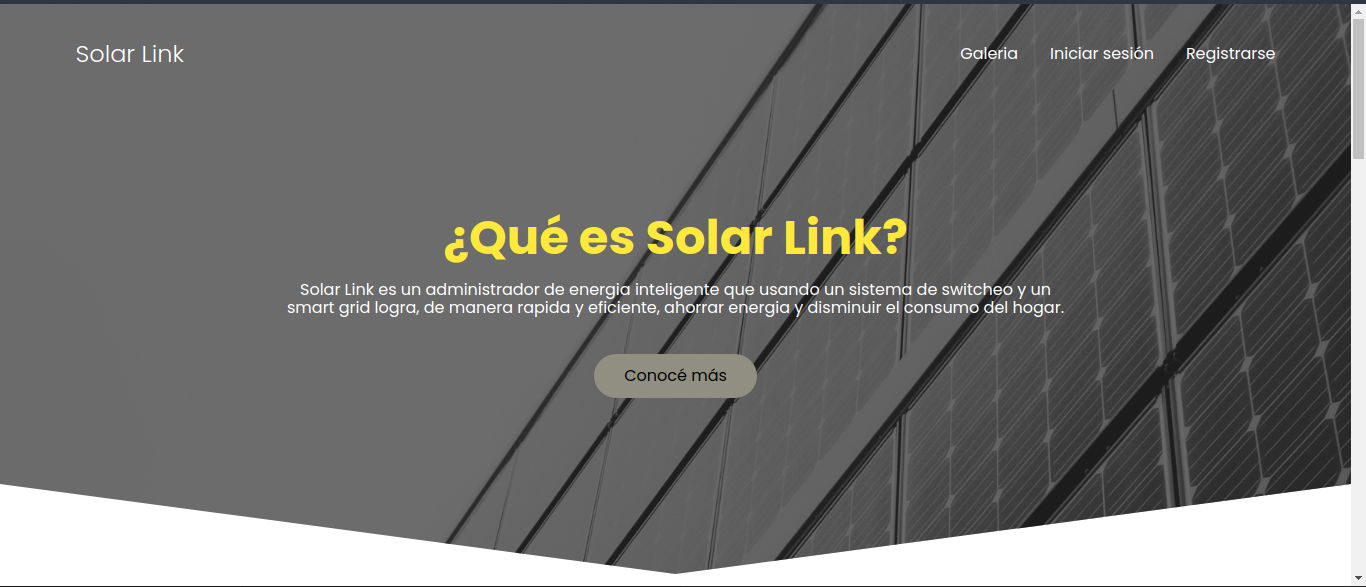
\includegraphics[width=1\linewidth]{web/Captura desde 2023-10-15 22-37-16.png}
    \caption{Pestaña principal para usuario sin loguear.}
    \label{fig:user-no-log}
\end{figure}

\begin{figure}[H]
    \centering
    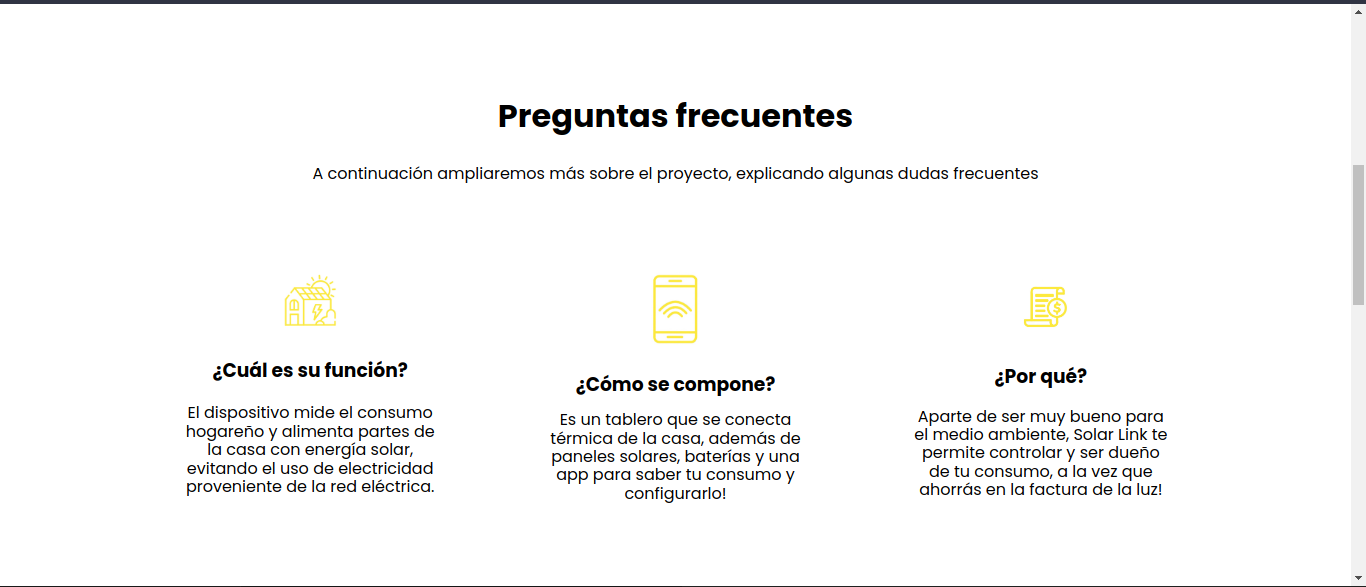
\includegraphics[width=1\linewidth]{web/Captura desde 2023-10-15 22-37-32.png}
    \caption{Pestaña de información del proyecto.}
    \label{fig:info-pry}
\end{figure}

\begin{figure}
    \centering
    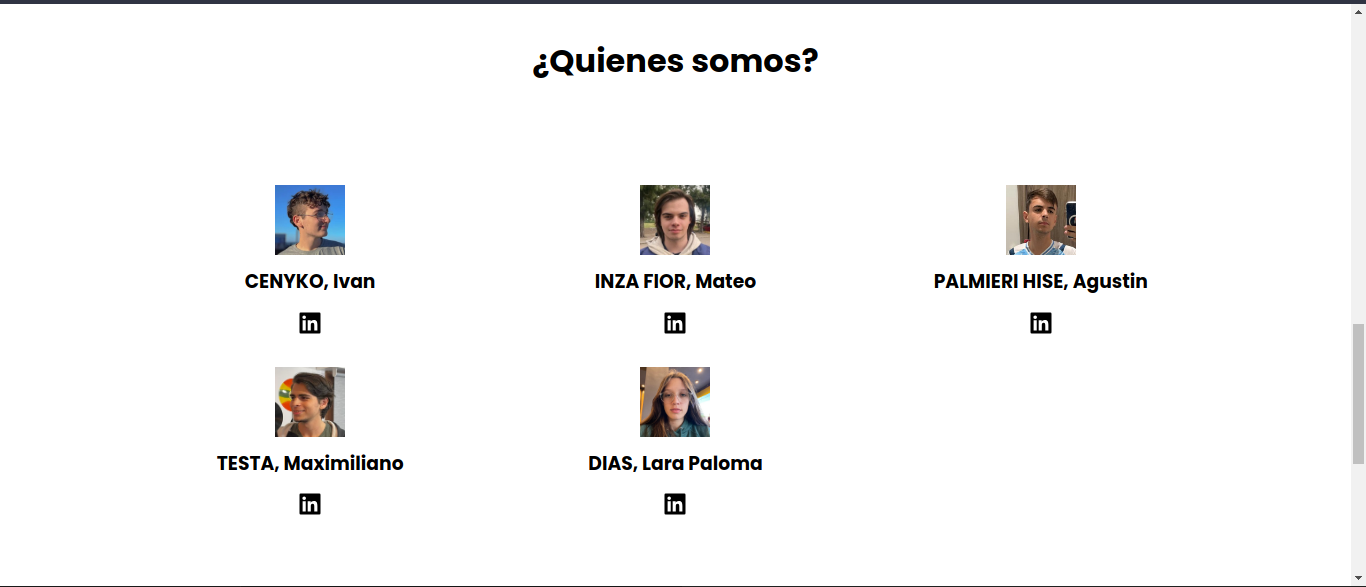
\includegraphics[width=1\linewidth]{web/Captura desde 2023-10-15 22-37-40.png}
    \caption{Pestaña de quienes somos.}
    \label{fig:quienes-somos}
\end{figure}

\begin{figure}[H]
    \centering
    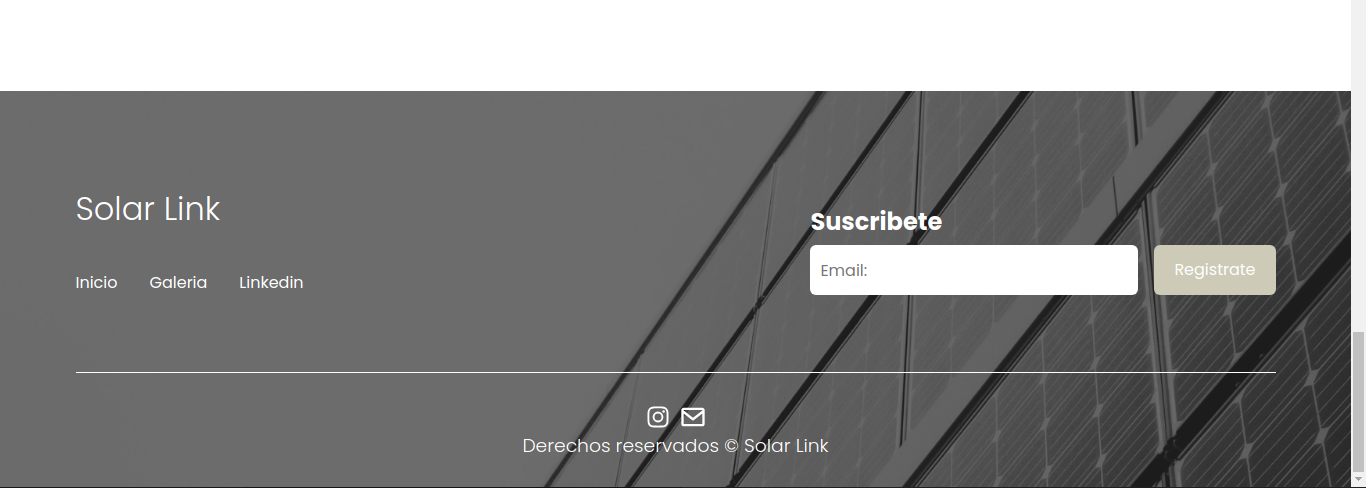
\includegraphics[width=1\linewidth]{web/Captura desde 2023-10-15 22-37-49.png}
    \caption{Pestaña para usuario sin loguear.}
    \label{fig:no-log-user}
\end{figure}

\begin{figure}[H]
    \centering
    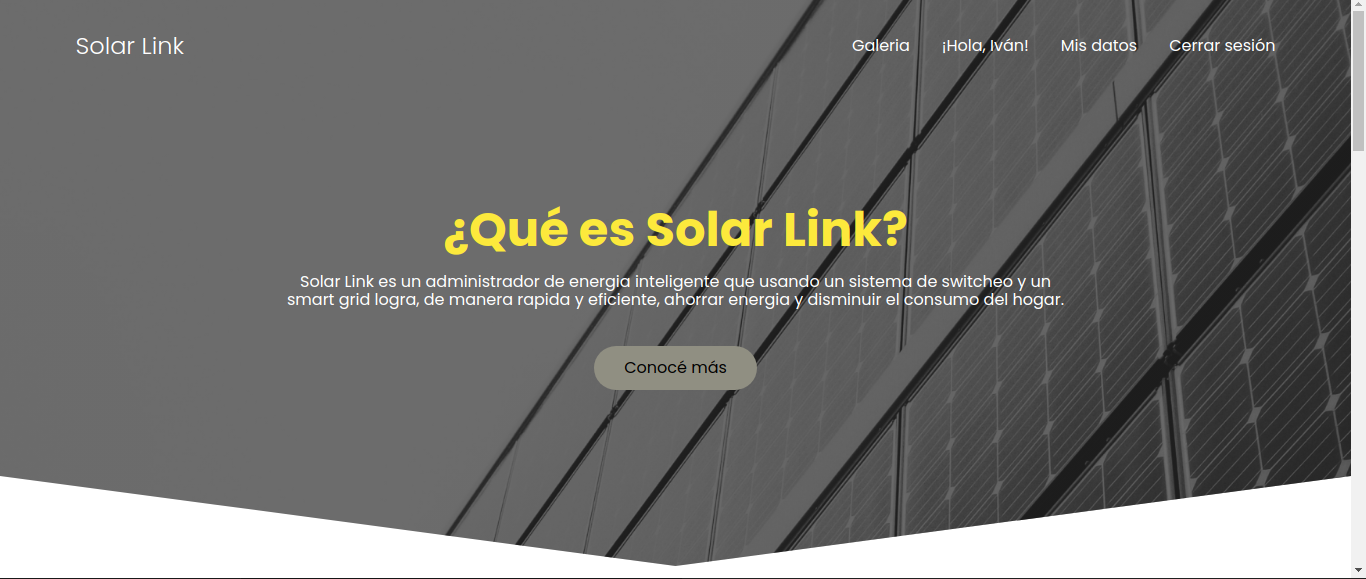
\includegraphics[width=1\linewidth]{web/Captura desde 2023-10-15 22-47-12.png}
    \caption{Pestaña de galería del proyecto.}
    \label{fig:galeria-web}
\end{figure}

\begin{figure}[H]
    \centering
    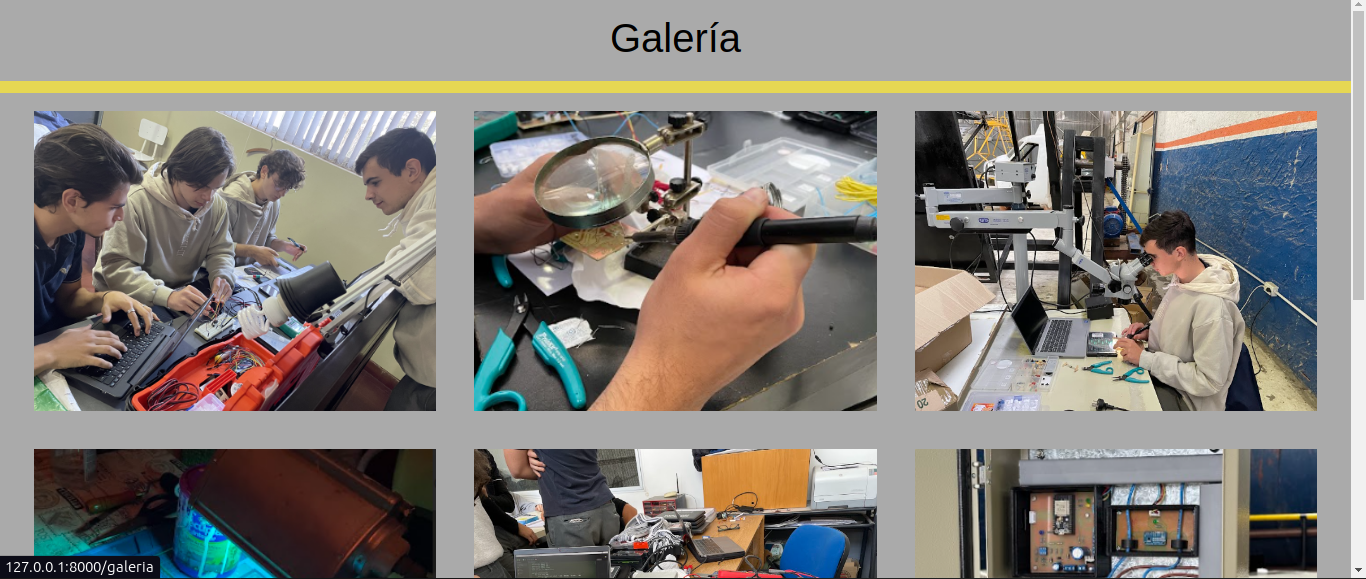
\includegraphics[width=0.8\linewidth]{web/Captura desde 2023-10-15 22-55-41.png}
    \caption{Pestaña galería.}
    \label{fig:user-log}
\end{figure}


\subsection{App User Managment}

\subsubsection{Directorio user\_mngmnt}
\begin{figure}[H]
    \centering
    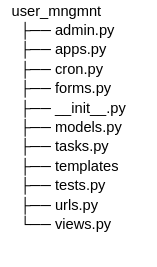
\includegraphics[width=0.25\linewidth]{web/Captura desde 2023-10-16 23-35-42.png}
    \caption{Directorio User Management.}
    \label{fig:dir-user_mngmnt}
\end{figure}
\begin{itemize}
    \item cron.py: contiene las funciones que se ejecutan cada cierto tiempo según la configuración de django-crontab.
    \item forms.py: contiene la configuración de los formularios web (como el de login, signup, etc).
    \item models.py: contiene los campos de la base de datos, concretamente hay tablas para los datos que sube el módulo Solar Link una vez por hora, el resumen de esos datos en formato diario, la llegada de datos en tiempo real (para cuando el usuario está viendo la pestaña de datos del módulo) y datos de emergencia (cuando surge algún problema en el módulo).
    \item tasks.py: contiene las tareas que se ejecutarán en un subproceso de celery.
    \item directorio templates: contiene los templates HTML de las distintas pestañas de user management, login, signup, etc.
    \item urls.py: al igual que en home, contiene los paths de las distintas pestañas o vistas.
    \item views.py: contiene la lógica de las vistas de esta app.
\end{itemize}

\subsubsection{Views}

En este views existen varias vistas:

\begin{itemize}
    \item Signup: Es la lógica de la vista de registro de usuarios, si se le hace un GET (por ejemplo desde el navegador) devuelve el template de registro renderizado con el formulario de signup (se explica en la sección de forms). Si se le hace un POST, revisa que el formulario sea válido, en caso contrario devuelve el mensaje de error correspondiente (como caracteres no válidos, contraseñas no coincidentes, etc). Si el registro es válido, crea el usuario, lo autentica,  crea un token de registro, y envía un mail con ese token para que el usuario confirme el registro y pueda acceder a la plataforma. En el listing \ref{signup_user_mngmnt} se encuentra el código.

\begin{figure}[H]

\begin{subfigure}{0.5\textwidth}
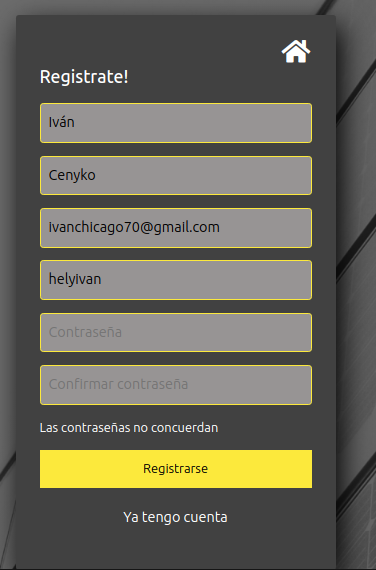
\includegraphics[width=0.9\linewidth]{web/Captura desde 2023-10-15 23-23-00.png} 
\caption{Las contraseñas no concuerdan.}
\label{fig:subim1}
\end{subfigure}
\begin{subfigure}{0.5\textwidth}
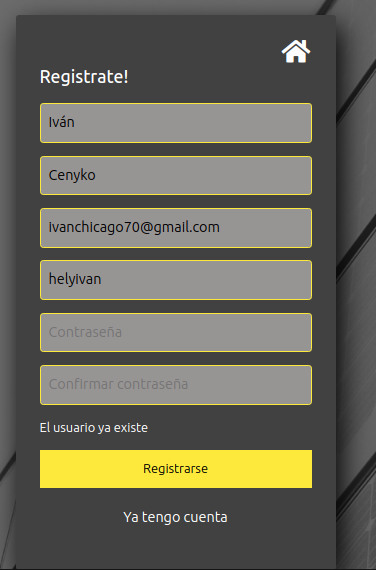
\includegraphics[width=0.9\linewidth]{web/Captura desde 2023-10-15 23-23-28.png}
\caption{El usuario ya existe.}
\label{fig:subim2}
\end{subfigure}

\caption{Casos de errores.}
\label{fig:image2}
\end{figure}

\begin{figure}[H]
    \centering
    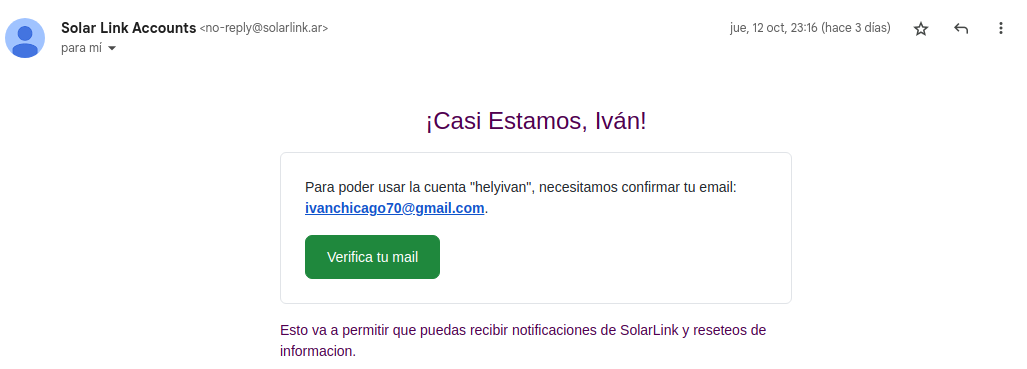
\includegraphics[width=1\linewidth]{web/Captura desde 2023-10-15 23-27-44.png}
    \caption{Mail de verificación de cuenta.}
    \label{fig:mail-verify}
\end{figure}

    \item Singup verification: Es la lógica que confirma al usuario cuando este pulsa el botón del mail de confirmación de registro. Básicamente revisa si existe el token del link, y si este está asociado al usuario. Si esas dos condiciones se cumplen, borra el token de la base de datos (para que no pueda ser reutilizado), activa al usuario, y envía un mail avisando al usuario que ya puede acceder a la plataforma. En el listing \ref{signup_verification_user_mngmnt} se detalla el código.

\begin{figure}[H]
    \centering
    
\includegraphics[width=1\linewidth]{web/Captura desde 2023-10-15 23-38-55.png}
    \caption{Verificación de cuenta exitoso.}
    \label{fig:mail-verify-ok}
\end{figure}
    
    \item Password reset: esta es la vista encargada de resetear la contraseña del usuario si se le otorga la dirección de correo adecuada. Si recibe un GET, devuelve la vista para pedir un cambio de contraseña. Si recibe un POST, genera un token para cada usuario asociado a ese mail, manda los mails de cambio de contraseña, y devuelve una vista confirmando el envío. En el listing \ref{password_reset_user_mngmnt} se detalla el código.

\begin{figure}[H]
    \centering
    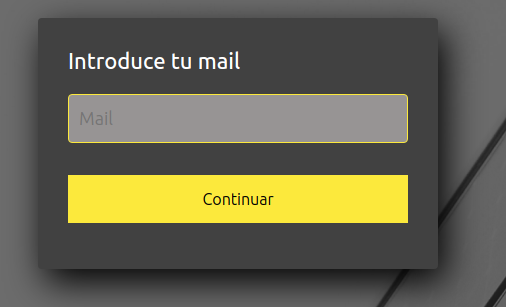
\includegraphics[width=0.7\linewidth]{web/Captura desde 2023-10-15 23-44-54.png}
    \caption{Pestaña de envío de mail.}
    \label{fig:introducir-mail}
\end{figure}

\begin{figure}[H]
    \centering
    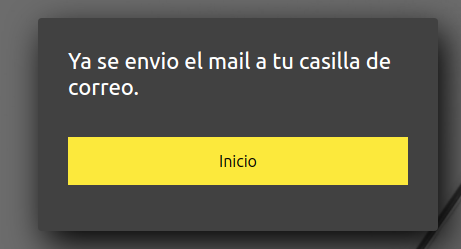
\includegraphics[width=0.7\linewidth]{web/Captura desde 2023-10-15 23-45-10.png}
    \caption{Aviso de envío de contraseña.}
    \label{fig:aviso-envio}
\end{figure}

\begin{figure}[H]
    \centering
    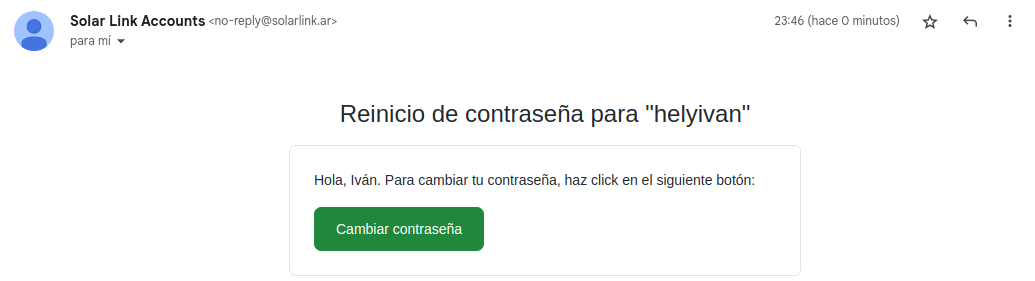
\includegraphics[width=1\linewidth]{web/Captura desde 2023-10-15 23-47-09.png}
    \caption{Mail de reinicio de contraseña.}
    \label{fig:reinicio-mail}
\end{figure}
    \item Password set: esta vista cambia la contraseña una vez ingresada la nueva por el usuario. Funciona de forma muy similar a SignupVerification, sólo que en lugar de habilitar al usuario, cambia su contraseña.
    \item Login: Si se accede con un GET, entrega el formulario de inicio de sesión para rellenar. Si se accede con un POST, revisa que el formulario sea válido, de serlo loguea al usuario y lo manda a la pestaña de datos. Caso contrario devuelve el código de error correspondiente. En el listing \ref{login_user_mngmnt} se detalla el código.

\begin{figure}[H]
    \centering
    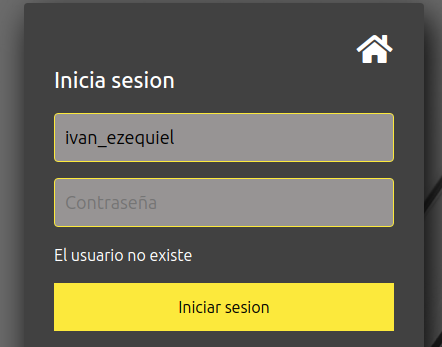
\includegraphics[width=0.7\linewidth]{web/Captura desde 2023-10-16 00-06-48.png}
    \caption{Caso de error donde el usuario no exista.}
    \label{fig:error-no-usuario}
\end{figure}
    
    \item Logout: Desloguea al usuario, solo se puede acceder si el usuario está logueado, por eso tiene el decorador login\_required. 
    
\end{itemize}

\subsubsection{Urls}
Aquí están los paths a todas las pestañas del views.py, puede notarse que está programado un decorador llamado unlogued required, este se encarga de hacer que las vistas a las que aplica solo sean accesibles por usuarios sin iniciar sesión, y se aplica en pestañas como la de login, en las que no resulta lógico que el usuario pueda acceder si ya está logueado. Luego se puede notar que muchas vistas tienen aplicada la función as view, esta se utiliza en aquellas vistas del views.py que están definidas como clase. Por último, existen dos vistas que tienen aplicado el csrf exempt, ya que django por defecto protege la página de POSTs indeseados con un sistema de cookies, que solo permiten POSTs provenientes de los formularios creados en forms.py, el decorador csrf exempt omite el pedido de cookies csrf para las vistas a las que se aplica, esto permite hacerle POSTs a la página desde afuera, concretamente desde la ESP32. En el listing \ref{urls.py_user_mngmnt} se encuentra el código.

\subsubsection{Forms}

Aquí se encuentran las clases que definen los formularios de inicio de sesión, registro, cambio de contraseña, etc. Se definen los campos (nombre, apellido, username, contraseña, etc). Y luego puede notarse que se define un método llamado clean para cada formulario. Este se encarga de devolver los mensajes de error, por ejemplo si el usuario ingresado no existe, si la contraseña es incorrecta, si las contraseñas en el registro no coinciden, etc. En el listing \ref{forms.py_user_mngmnt} se encuentra el código de la clase del login, a forma de ejemplo.

\subsubsection{Cron}

Aquí se definen dos tareas que se ejecutan periódicamente. Una se encarga de tomar todos los datos subidos en el dia por cada usuario, acumularlos en un dato único diario en otra tabla de la base de datos, y borrar los datos subidos por hora; esto se hace para no sobrecargar la base de datos de información, se ejecuta una vez por día. Luego existe otra tarea que se ejecuta cada 10 minutos, y se encarga de borrar los tokens de registro o cambio de contraseña que se hayan creado hace 2 horas o más, para que no representen una vulnerabilidad en el sistema. En el listing \ref{algoritmo_sorter_user_mngmnt} se muestra el algoritmo que revisa los datos de cada usuario y los acumula, y en el listing \ref{algoritmo_borra_tokens_user_mngmnt} la función borra tokens.

\subsubsection{Models}

Aquí se definen los campos y tablas de la base de datos. Varias funcionan con foreign keys, que asocian varios datos de una tabla con los datos de otra. Concretamente, vinculan los datos subidos con un usuario, que está almacenado en la tabla de Users. También tienen definida una subclase llamada Meta, que se encarga de que los datos se lean ordenados por fecha y por usuario. En el listing \ref{models.py_DatosHora_user_mngmnt} se encuentra el modelo de la tabla de datos que se suben por hora, a modo de ejemplo. 

\subsubsection{Tasks}

Aquí se definen las tareas que se quieren ejecutar en subprocesos de Celery. Se definió que los mails se ejecuten en un subproceso, ya que pueden tomar tiempo en enviarse, y el objetivo es que la pestaña sea lo más rápida posible. Entonces, la pestaña envía un pedido de subproceso para enviar mails a Celery, y devuelve rápidamente el HTML correspondiente a esa pestaña, sin una demora ante la perspectiva del usuario. En el listing \ref{tasks.py_mails_user_mngmnt} se muestra el código de esa función subproceso. En las configuraciones (listing \ref{settings.py}) se puede ver la dirección de correo \href{no-reply@solarlink.ar}{no-reply@solarlink.ar}, que es la que se usa para enviar los mails de confirmación de registro y cambio de contraseña con el protocolo SMTP (permite, entre otras cosas, enviar mails desde el backend del proyecto); como así las configuraciones de Zoho, el servidor de mails utilizado.

\subsubsection{Directorio templates}
\begin{figure}[H]
    \centering
    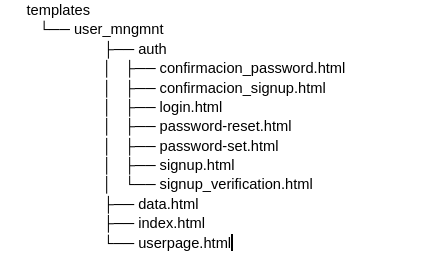
\includegraphics[width=0.7\linewidth]{web/Captura desde 2023-10-17 00-12-42.png}
    \caption{Directorio templates de User Management.}
    \label{fig:dir-templates_user_mngmnt}
\end{figure}
Aquí se encuentran los templates HTML para las pestañas de login, signup, confirmación de registro y cambio de contraseña, los mails, etc. A continuación imágenes del diseño final.

\begin{figure}[H]
    \centering
    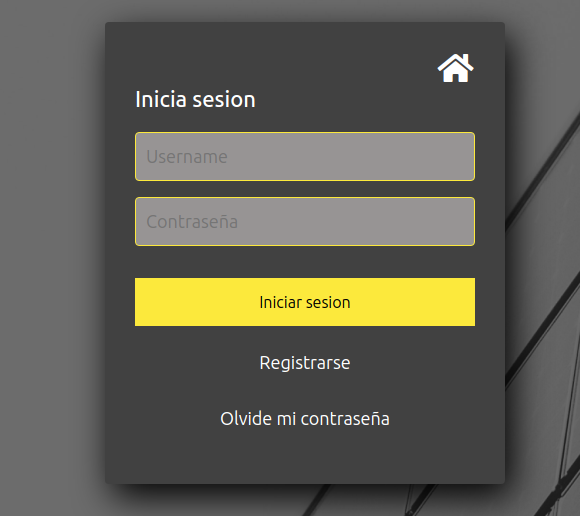
\includegraphics[width=0.60\linewidth]{web/Captura desde 2023-10-16 21-28-23.png}
    \caption{Diseño del login.}
    \label{fig:enter-label}
\end{figure}

\begin{figure}[H]
    \centering
    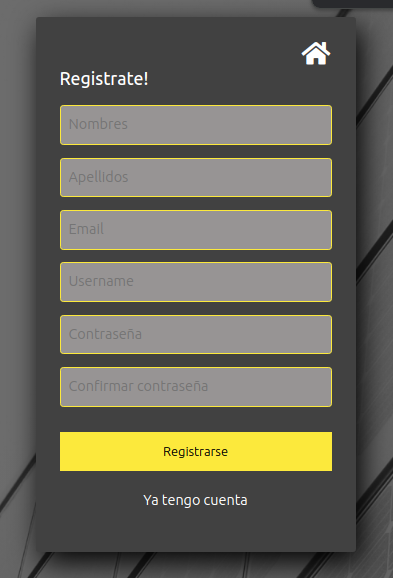
\includegraphics[width=0.5\linewidth]{web/Captura desde 2023-10-16 21-28-51.png}
    \caption{Diseño del registro.}
    \label{fig:enter-label}
\end{figure}

\begin{figure}[H]
    \centering
    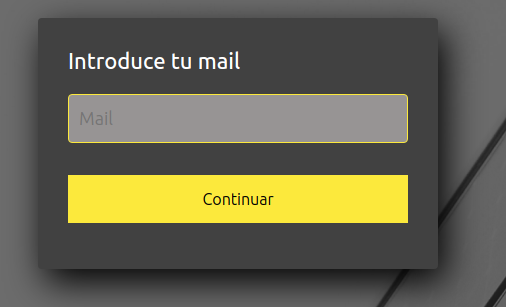
\includegraphics[width=1\linewidth]{web/Captura desde 2023-10-15 23-44-54.png}
    \caption{Diseño del cambio de contraseña.}
    \label{fig:enter-label}
\end{figure}

\begin{figure}[H]
    \centering
    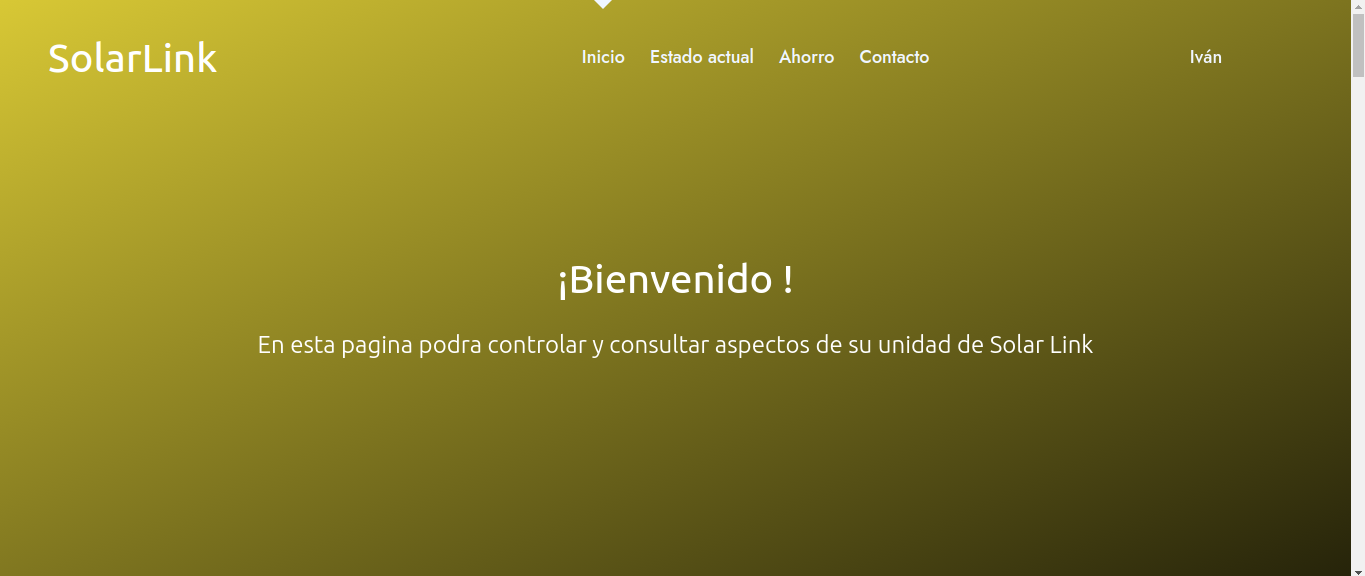
\includegraphics[width=1\linewidth]{web/Captura desde 2023-10-16 21-30-19.png}
    \caption{Parte superior de la página de datos.}
    \label{fig:enter-label}
\end{figure}

\begin{figure}[H]
    \centering
    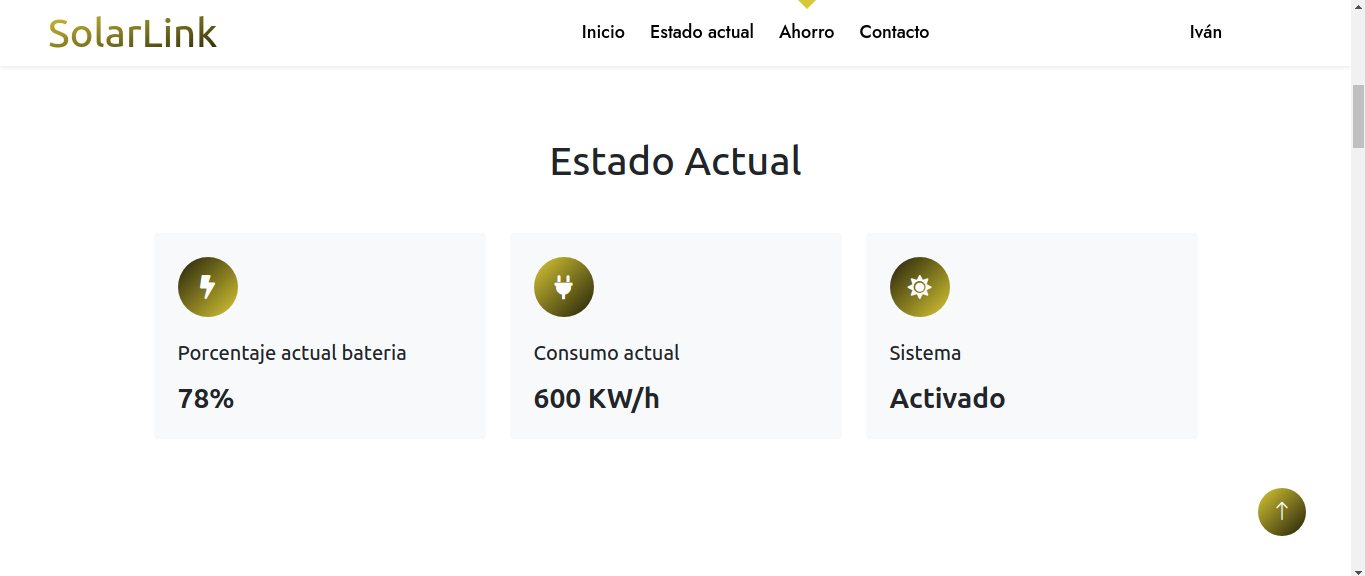
\includegraphics[width=1\linewidth]{web/Captura desde 2023-10-16 21-30-33.png}
    \caption{Estado actual.}
    \label{fig:enter-label}
\end{figure}

\begin{figure}[H]
    \centering
    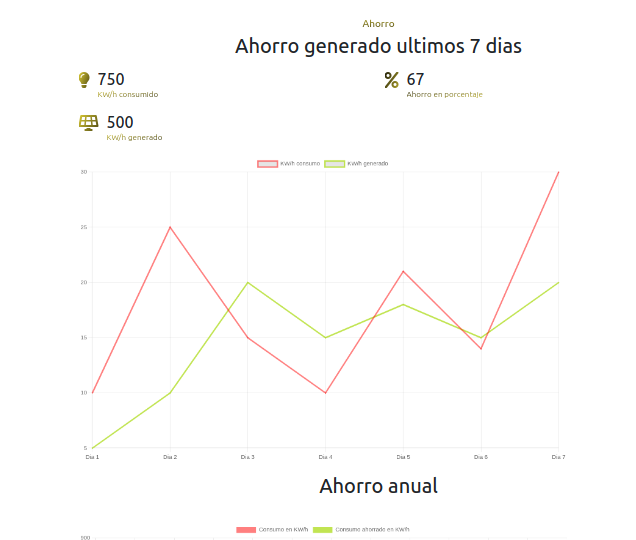
\includegraphics[width=0.75\linewidth]{web/Captura desde 2023-10-16 21-30-55.png}
    \caption{Gráficas ahorro semanal.}
    \label{fig:enter-label}
\end{figure}

\begin{figure}[H]
    \centering
    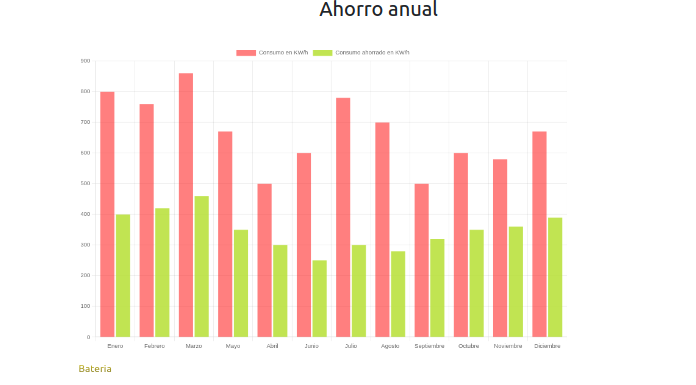
\includegraphics[width=1\linewidth]{web/Captura desde 2023-10-16 21-31-11.png}
    \caption{Ahorro anual.}
    \label{fig:enter-label}
\end{figure}

\begin{figure}[H]
    \centering
    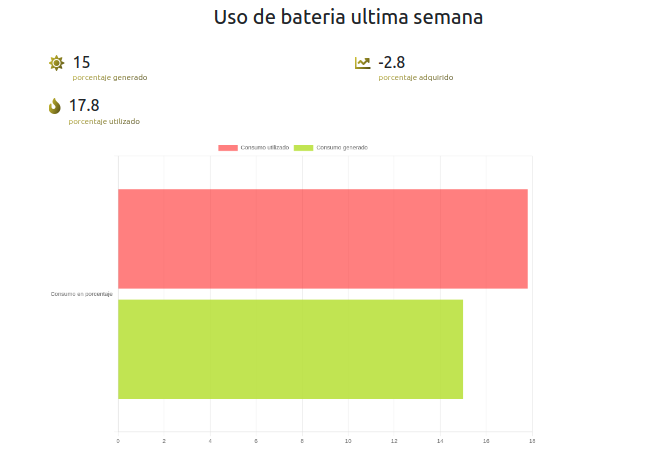
\includegraphics[width=0.75\linewidth]{web/Captura desde 2023-10-16 21-31-23.png}
    \caption{Uso de la batería en la última semana.}
    \label{fig:enter-label}
\end{figure}

\subsection{Hosting de Vercel}
Para la página web necesitábamos un hosting. Nos decantamos por Vercel debido a que es de los pocos hosting gratuitos que soportaba el desarrollo web en python-django, aparte que tiene un método de deploys muy sencillo, que consiste en que toma una branch del repositorio de GitHub proporcionado, y la usa como raíz para la página web; cada push a esa branch es un nuevo deploy que actualiza la página web. Para funcionar, sólo requiere dos archivos específicos en el directorio raíz: un vercel.json que le indique qué tipo de lenguaje y framework usa la web, y un requirements.txt para saber qué modulos de python instalar. En los listings \ref{vercel.json} y \ref{requirements.txt} se muestran esos archivos respectivamente.

\begin{figure}[H]
    \centering
    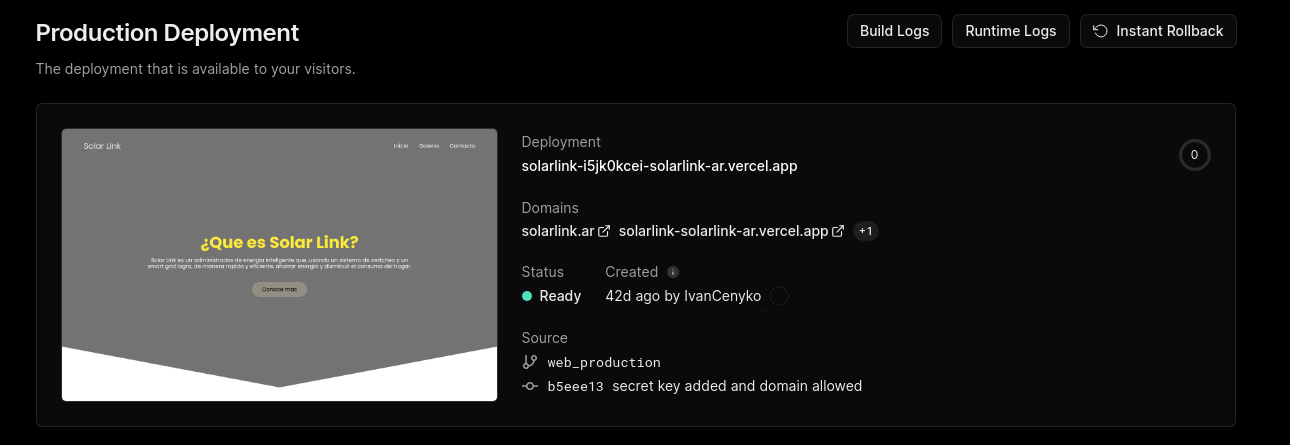
\includegraphics[width=1.2\linewidth]{web/Captura desde 2023-10-17 15-49-12.png}
    \caption{Ejemplo de deploy de vercel}
    \label{fig:enter-label}
\end{figure}

Aquí también se configuró el DNS con el dominio que compramos \href{https://solarlink.ar}{solarlink.ar} y los accesos al servicio Zoho, que nos permitió tener mails de dominio propio como \href{info@solarlink.ar}{info@solarlink.ar} y \href{no-reply@solarlink.ar}{no-reply@solarlink.ar}  .
\begin{figure}[H]
    \centering
    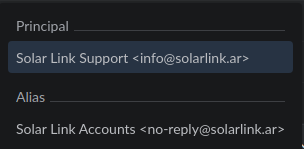
\includegraphics[width=0.5\linewidth]{web/Captura desde 2023-10-17 16-45-31.png}
    \caption{Mails configurados en Zoho}
    \label{fig:zoho mail}
\end{figure}